\section{SOAR Platform Components}

A Security Orchestration, Automation, and Response (SOAR) solution is commonly made up of many different modules that are useful for primary phases of the incident response life cycle, ranging from ingestion and detection all the way through to analysis, orchestration, and resolution. According to Gartner, SOAR platforms bring together security operations by using playbook-driven automation, workflow orchestration, case management and integration with third-party tools and services~\cite{gartner-siem-soar}. These platforms aim to help SOC analysts by relieving them from repetitive tasks, using consistent responses and documenting their work to ensure auditability.

Commercial standard SOAR solutions, like Splunk SOAR (formerly Phantom) and Palo Alto Cortex XSOAR, provide a myriad of modules for incident handling, playbook execution and third-party integration ~\cite{splunk, paloalto}. For example, Splunk SOAR has a visual playbook builder, a case management tool, over 300 prebuilt integration options (called apps), and a detailed REST API solution for system integration~\cite{splunk}. SimilSimilarly, Palo Alto XSOAR offers integrated case and incident visibility, MITRE ATT\&CK based incident tagging and a marketplace for streamlined extensibility ~\cite{paloalto}. Open-source options, including Shuffle, also offer many capabilities, as well as lightweight, easy-to-use visual automation experiences with pluggable REST actions and community built workflows~\cite{techtarget}.

Although there are some minor differences (in the details) on how SOAR will be implemented, the vast majority of SOAR tools leverage a modular architecture composed of reusable components. Often times these components include:

\begin{itemize}
    \item \textbf{Authentication and User Management:} The authentication and user management component provides authentication, access management and user provisioning. In enterprise SOAR platforms this module is often integrated with SSO, LDAP, or SAML identity providers for central identity management.
    
    \item \textbf{Dashboard and Analytics:} The dashboard and analytics component provides users with a single pane of glass that illustrates trends in incidents or use metrics that can be displayed in charts or graphs, such as pie charts, bar charts, and time series visuals. Dashboards are used by SOC managers when they need assistance in planning and operational oversight~\cite{paloalto}.

    \item \textbf{Incident Management:} The incident management component is the central module used for gathering, reviewing and taking action on alerts generated from SIEM, threat intelligence feeds, or manual sources. Incidents will often contain metadata such as source IPs, attack vectors, severity level, and mappings to the MITRE ATT\&CK framework.

    \item \textbf{Integrations:} The integrations component refers to the ability to integrate with external security and IT tools (e.g., firewalls, EDRs, ticketing systems, threat intel platforms). Integrations are often expressed as “apps” or “connectors” or something similar that plug into the SOAR tool and enable an action like, for example, the ability to send an action to a ticketing system through a REST API, which can be an example of bi-directional communication and orchestration~\cite{techtarget}.

    \item \textbf{Playbooks:} Use a flow-based definition of the logic for an automated response. Playbooks can be triggered by the type of incident or rules. Playbooks allow executing actions, including notified and enrichment of information, containment, and notifications within a sequence. Playbooks can ensure consistency and repeatability in incident handling~\cite{splunk, paloalto}.

    \item \textbf{Workflow Engine:} Provides a visual or low-code interface allowing actions and conditions to be linked in an executable sequence. Some SOAR platforms (i.e., Shuffle) allow workflows to be created with drag and drop actions in place to offer better usability with lower code reliance~\cite{techtarget}.

    \item \textbf{Case Management and Audit Trails:} Allow analysts to monitor the situation, document their decisions, and maintain, full auditability of their response (potentially also fulfill compliance/classification requirements), and for use in a post-mortem analysis. Important in restricted sectors (finance and defence).

    \item \textbf{MITRE ATT\&CK Integration:} A large majority of modern SOAR platforms are now incorporating the MITRE ATT\&CK framework, which provides categorization of incidents based on tactics and techniques. This helps with the strategic mapping of threats, and helps incidents be correlated and prioritized for actions taken~\cite{mitre}.
\end{itemize}

All of these elements are essential to automatically manage the incident lifecycle, reduce analyst fatigue, and decrease the mean time to respond (MTTR). Commercial platforms provide advanced implementations, but the custom SOAR solutions can be configured to satisfy distinct organizational and regulatory considerations, such as air-gapped environments in national defense infrastructures.

\subsection{User Authentication}

The user authentication implemented with the help of \textbf{Login and Signup} module is the entry point into the SOAR platform, responsible for identifying users and managing their access rights. The operations that are undertaken in the SOAR environment are important and sensitive in nature (e.g. accessing threat intelligence, executing playbooks, incident responses); thus, the user authentication module must be secure and possess functionality that relates to user management. Hence, the module must be designed to prevent unauthorized access, ensure data integrity, and provide a seamless user experience.

In the implemented system, users register with unique username and password that are stored securely in the backend database. Passwords are never written in plain text. When a user registers, their password will be hashed with a cryptographic hash function (like SHA-256 or bcrypt). When a user logs in, the login password is securely compared to the entries in the database (using secure comparison) to ensure that it is not vulnerable to timing attacks.

The authentication mechanism is stateless and uses session cookies to persist the user state, post-login. After authentication, the user receives a token that must be produced with future APIs. This token based implementation is standard practice in the field, due to the scalability benefits and secure sessions~\cite{paloalto, techtarget}. The token is signed and can be verified by the server to ensure its authenticity. The token also contains user information, such as user ID and roles, which can be used for authorization.

Currently, the implementation only supports single-role authentication, but the architecture allows for Role-Based Access Control (RBAC) in the future. This is useful when establishing role-based access of specialist teams to certain modules, like, incident response, playbook management, and integrations for operational security and accountability. Different roles can be assigned to users, such as SOC analyst, SOC manager, or administrator, each with different permissions and access levels.

In comparison, enterprise-grade SOAR platforms like Splunk SOAR, and Palo Alto (XSOAR) provide advanced authentication features, including Single Sign-On (SSO), integration to the Lightweight Directory Access Protocol (LDAP), Security Assertion Markup Language (SAML), and multi-factor authentication (MFA)~\cite{splunk, paloalto}. While these features are important to large organizations, lightweight and locally-hosted SOAR solutions may have uuid or token based credentials to provide an easier way of managing access to the solution, especially when handling deployed solutions in air gapped and restricted environments, like defense organizations.

In summary, the Login/Signup module in the developed SOAR system provides both a secure and extensible platform for user authentication. It ensures that only authorized users have access to sensitive features in the system. The module is modular and may allow for future improvements, such as access auditing, multi-factor authentication (MFA), or integration with national identity providers.

\subsection{Dashboard}

The \textbf{Dashboard} acts as the single visualization platform of SOAR providing SOC analysts and administrators with the capability to view the near real-time status of the security  environment. The Dashboard reduces the amount of span of control, identifying the situation  regarding ongoing incidents, trends with incidents over time, and response metrics.  Dashboards are effective for operational situational awareness, strategic planning and post-event analysis.

\begin{figure}[ht]
    \centering
    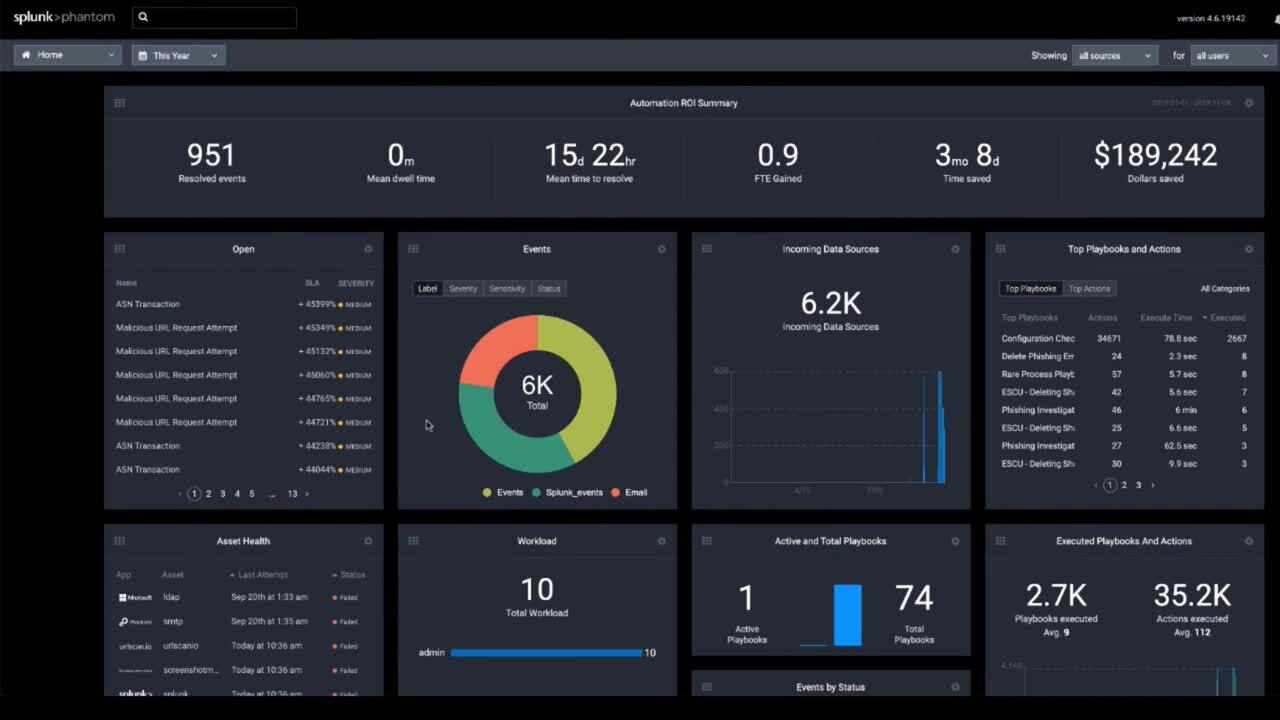
\includegraphics[width=0.9\textwidth]{images/splunk_soar_dashboard.jpg}
    \caption[Example of a Splunk SOAR dashboard]{Example of a Splunk SOAR dashboard. Such dashboards provide SOC teams with real-time visibility into security operations and response effectiveness.}
    \label{fig:splunk-soar-dashboard}
\end{figure}

In the implemented SOAR system, the dashboard consists of multiple interactive visual components:

\begin{itemize}[noitemsep,topsep=0pt]
    \item \textbf{Pie Charts:} Represent incident breaks down by severity (e.g., low, medium, high, critical) and status (e.g., open, in-progress, mitigated, closed). 
    \item \textbf{Stacked Area Chart:} Demonstrates the time-based trend of incidents in each category, allowing for incidences of peaks and valleys in reporting over time. 
    \item \textbf{Bar Graph:} It displays the top attack types or event categories based on frequency, that helps in prioritizing the detection rules and playbook tuning.
    \item \textbf{Line Graph:} Displays overall incident volume over time; useful for detecting recurring patterns that signify a threat or an anomaly in network behavior.
    \item \textbf{Mitigated Incidents Table:} A table describing resolved incidents over time.  Each incident is listed with a timestamp, severity of the incident, method of mitigation, and notes from analyst.
\end{itemize}

The visualizations are generated dynamically from the backend database so that the SOC team has the most current information. As new front-end technologies allow for filtering, hovering on the graphics, and drill-down capabilities, they make these more accessible for Tier 1 analysts and SOC managers.

By comparison, enterprise-grade SOAR platforms like \textbf{Splunk SOAR} and \textbf{Palo Alto} Cortex XSOAR also feature strong dashboard modules. The Splunk SOAR dashboard includes customizable widgets, that show the automation coverage, stats on playbook executions, case resolution times, and breakdown of type of threat~\cite{splunk}. XSOAR provides executive summary views, threat intelligence overlays, SLA view and integrates with MITRE ATT\&CK matrix visualizations~\cite{paloalto}. These features assist high-level directors with monitoring the security posture, compliance compliance, and operational performance at scale.

Open-source platforms like \textbf{Shuffle} present a more lightweight example where the dashboard provides basic content and a within the dashboard presents execution success rates, most recent runs, and tasks that have failed~\cite{techtarget}. In comparison to commercial platforms mentioned earlier, it is minimal, but can be extended using third-party tools such as Grafana or Kibana for increased visibility.

The inclusion of a comprehensive dashboard module is an important function for supporting data-driven incident response. By implementing a dashboard, the SOC can monitor KPIs such as Mean Time to Detect (MTTD) and Mean Time to Respond (MTTR). It can also identify bottlenecks, repeatable alerts, and areas of playbook coverage inadequacies. A high-quality incident response dashboard converts data into useful, actionable insight that can help the SOC to improve operational maturity through continuous improvement.

\subsection{Incidents}

The Incidents module is the operation core of the SOAR platform, and the direct consumer of alerts received directly from upstream systems like a Security Information and Event Management (SIEM) system. The alerts are correlated and determined to be actionable; they are stored as incidents in the incident management system where analysts can open and investigate incidents interactively through structured interfaces and automated workflows.

The SOAR system that has been implemented displays incidents in an interactive and filterable table. Each row describes a single incident, that may contain the following metadata fields:

\begin{itemize}[noitemsep,topsep=0pt]
    \item \textbf{Timestamp:} The time at which the incident was triggered.
    \item \textbf{Attack Type:} Categorization based on the detected behavior (e.g., brute-force, phishing, malware).
    \item \textbf{Severity:} A rating (e.g., low, medium, high, critical) based on correlation rules or risk score.
    \item \textbf{Source and Destination IPs/Hosts:} Network location of the event.
    \item \textbf{Associated MITRE Technique IDs:} Tactic and technique labels for threat classification.
    \item \textbf{Status:} Indicates whether the incident is open, in progress, resolved, or closed.
\end{itemize}

Users can use filters to select which incidents they want to view by attack type, status, or severity and take response actions from the interface itself. A unique feature of this platform is that it allows both manual and AI-assisted updates to incident status. Analysts have the option to either take manual actions, such as marking an incident as mitigated, or request mitigation recommendations stepped out by a selected ML model, which recommends based on past resolutions. 

\begin{figure}[ht]
    \centering
    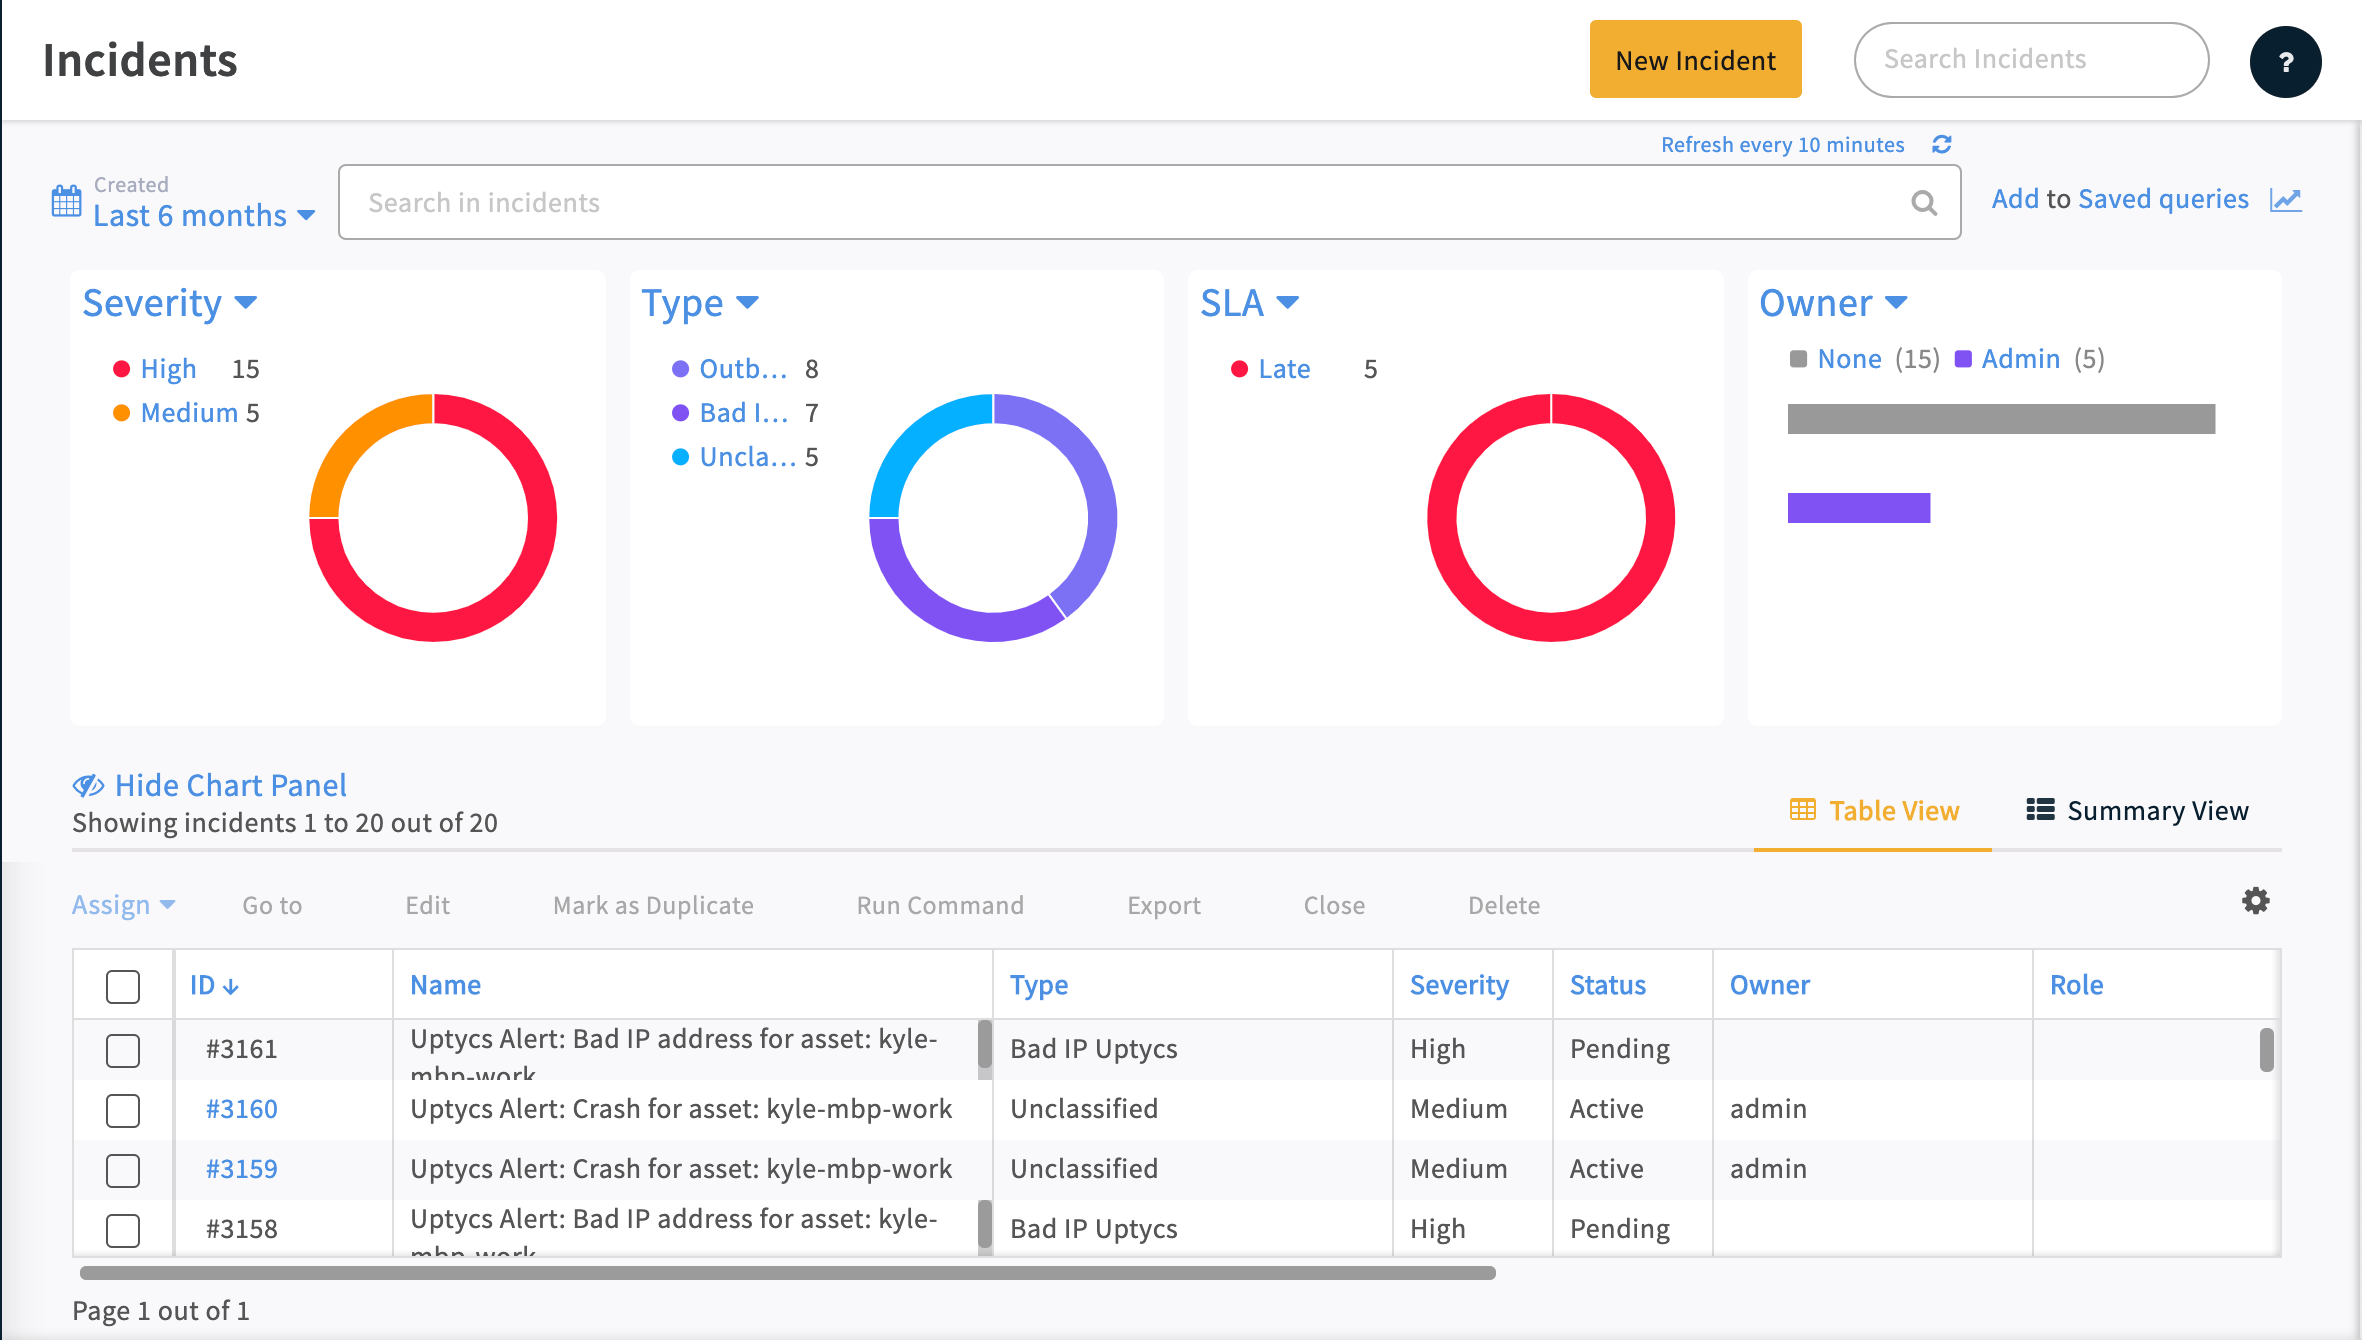
\includegraphics[width=0.9\textwidth]{images/xsoar_incidents.png}
    \caption[Incident management interface in Palo Alto Cortex XSOAR]{Incident management interface in Palo Alto Cortex XSOAR. The interface provides analysts with a comprehensive view of incidents, including filtering, status updates, and detailed metadata for each alert.}
    \label{fig:xsoar-incidents}
\end{figure}

This AI-assisted mitigation capability surpasses the present capabilities of many commercial SOAR platforms, where features include AI-ML to some extent, or is at least limited as an external integration; examples include Splunk SOAR, which provides advanced correlation and playbook automation, but does not inherently provides for ML model selection for selecting self-learned response, without having integrated third-party platforms~\cite{splunk}; and Cortex XSOAR provides for data enrichment and contextual awareness, but with its machine learning features, relies on Palo Alto’s Threat Intelligence, or other external resources~\cite{paloalto}.

Open-source SOAR tools such as Shuffle provide a rather coarse incident ingestion and display process from webhook integrations, but without native enrichment, severity-scoring, or AI-assisted resolution workflows~\cite{techtarget}. The presented SOAR system thus bridges this gap by offering native ML model selection for predictive mitigation, making it suitable for organizations that want to experiment with or deploy AI-driven security automation.

In conclusion, the incident module in the custom SOAR platform not only visualizes threat data but actively integrates with intelligence, analytics, and automation components. Its hybrid approach—combining analyst control with AI support—ensures scalability, consistency, and reduced mean time to respond (MTTR) in SOC operations.

\subsection{Integrations}

The Integrations module is the building block of any SOAR platform allowing it to connect and orchestrate a diverse set of cyber security tools and systems within an ecosystem. It enables the platform to communicate with other vendor tools/resources (i.e. firewall, EPP/EDR, threat intelligence feeds, vulnerability scanners, cloud providers, ticketing systems, etc.) using standardized API interfaces. This connectivity is important to allow an automated action to be performed during the execution of a playbook or as part of manual analyst workflow. 

In the implemented SOAR platform, integrations are managed through a interface that provides the option of creating, modifying and deleting Apps and Actions:

\begin{itemize}[noitemsep,topsep=0pt]
    \item \textbf{App:} Represents an internal or external service or tool. Each app in the platform has fields for name, description, and API token.
    \item \textbf{Action:} Represents a specific action that can be performed by the app. Each action has fields for action name, HTTP method (GET, POST, PUT, DELETE), and the associated API endpoint URL.
\end{itemize}

The defined actions allow non-technical users to register integrations and use them across various workflows without writing code. Once configured, the actions can either be triggered via playbooks, or performed manually from the incident module. For example, a configured VirusTotal app may have actions like ‘scan\_url‘, ‘check\_hash‘, or ‘get\_report‘, and can be invoked during the threat enrichment stage.

Compared to commercial solutions, this modular app-action model is aligned with industry best practices. Splunk SOAR, for instance, provides over 300 built-in integrations known as “apps,” each containing a set of pre-configured actions. These can be used in visual playbooks and extended via custom Python scripting~\cite{splunk}. Similarly, Cortex XSOAR organizes integrations into packs that include playbook tasks, data models, and API-based connectors~\cite{paloalto}. It also supports live configuration from the user interface and centralized credential management.

Open-source platforms such as Shuffle follow a comparable model by offering REST-based integrations that can be created or imported from community repositories. Shuffle also allows users to write lightweight custom apps in Python or JavaScript, which are run in sandboxed Docker containers ~\cite{techtarget}.

\begin{figure}[ht]
    \centering
    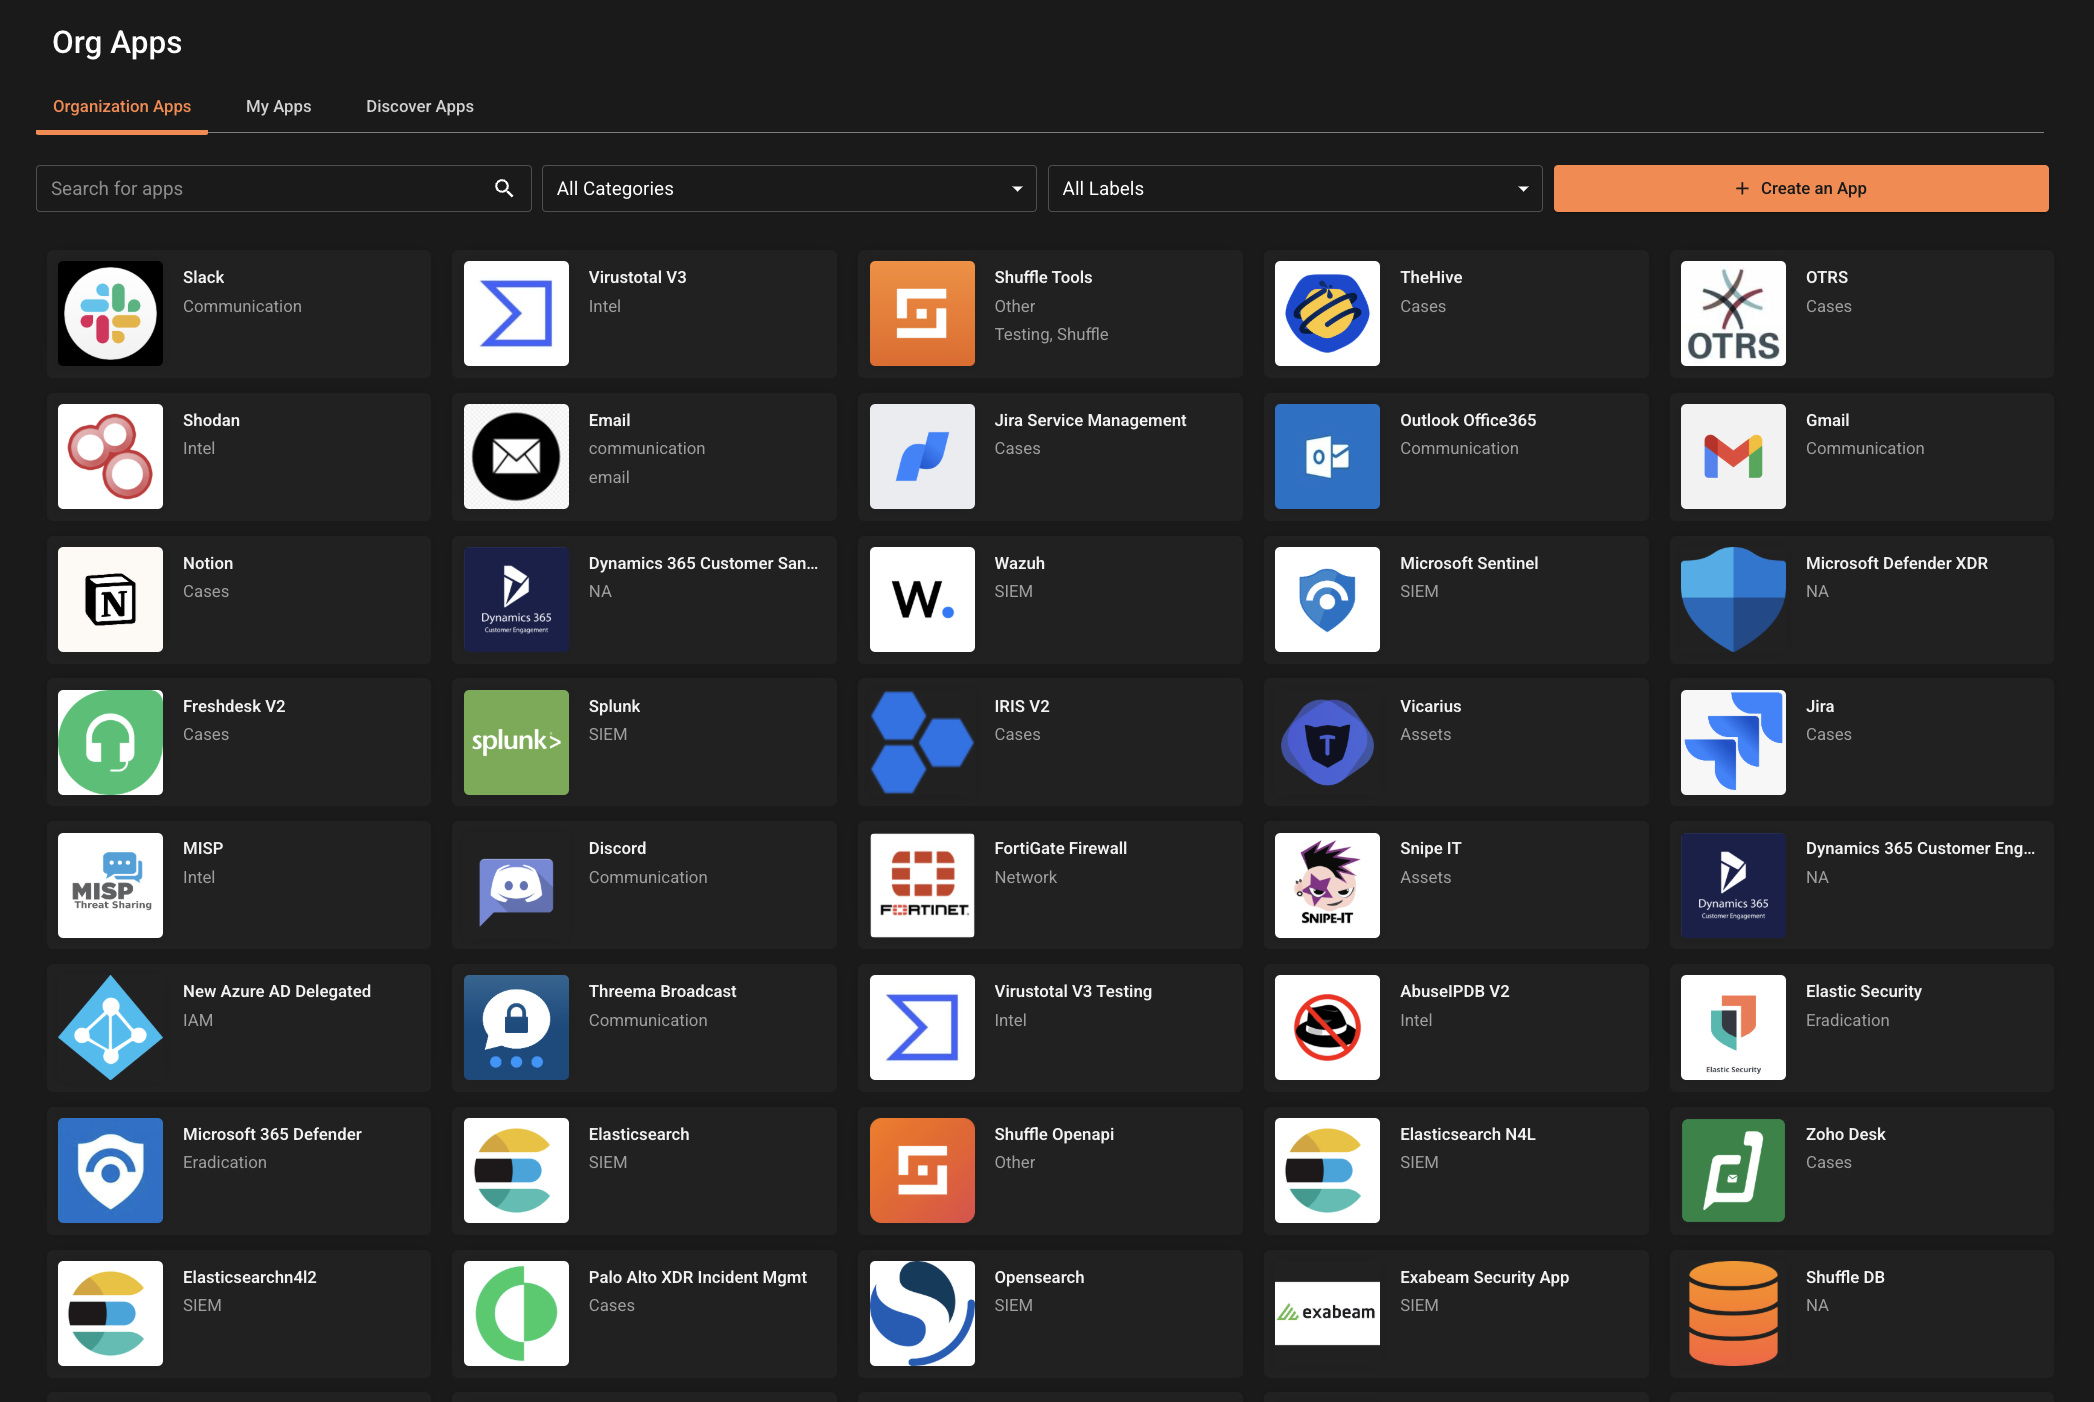
\includegraphics[width=0.9\textwidth]{images/shuffle_soar_apps.png}
    \caption[Example of the integrations (apps) interface in Shuffle SOAR]{Example of the integrations (apps) interface in Shuffle SOAR. Users can visually manage and configure third-party integrations and their actions through a web-based UI.}
    \label{fig:shuffle-soar-apps}
\end{figure}

The integrations module not only increases automation, but provides scalability and modularity in security operations. Each external service can be treated as a pluggable app with configurable actions, so the platform follows the principles of microservices, giving future orchestrations extensibility.

\subsection{Playbooks}

The Playbooks module acts as the automation engine for the SOAR platform, allowing structured, repeatable responses to security incidents, once detected. A playbook is the definition of the steps (both automated and manual) involved in how to investigate and remediate an incident. Playbooks are advantageous because they assist with consistency and stains by reducing analyst fatigue and reducing human mistake in a heavy volume environment.

In the SOAR system that was implemented, playbooks can be defined, managed, and construed from an intuitive user interface. The nucleus features of the module are:

\begin{itemize}[noitemsep,topsep=0pt]
    \item \textbf{Add/Edit/Delete Playbook:} The user can create playbooks, and/or edit or change playbooks as the procedures or types of threat and/or compliance change.
    
    \item \textbf{MITRE ATT\&CK Association:} Each playbook can be associated with one or more MITRE ATT\&CK Technique IDs. The playbook is automatically initiated in response to incoming incidents tagged with a technique identifier. This has the added benefit of allowing for context-aware, tactic-specific response automation~\cite{mitre}.
    
    \item \textbf{Workflow Linking:} Playbooks are associated with workflows—graphical flows that indicate the sequence of actions and conditions to instantiate. This allows users to have the logical decision-making layer (playbooks) and execution engine (workflow) decoupled, promoting reusability and flexibility.
\end{itemize}

The logic defined within a playbook may include other response actions, such as:
\begin{itemize}[noitemsep,topsep=0pt]
    \item Enriching indicators with threat intelligence sources (e.g., WHOIS, VirusTotal).
    \item Blocking malicious IP addresses or URLs by integrating with firewalls or web gateways.
    \item Isolating endpoints using an EDR (e.g., Crowdstrike or DarkTrace).
    \item Opening tickets or notifications through ticketing systems or email platforms.
\end{itemize}

Each of the steps may have conditions, triggers, and optional human approvals that allow playbooks to operate in fully automated or semi-automated modes.

This way of implementing uses the design philosophy of enterprise-level SOAR platforms; for example, Splunk SOAR supports building playbooks with a visual editor that utilizes decision blocks, automation tasks, and manual inputs~\cite{splunk}. Although Splunk SOAR playbooks use Python internally, they are abstracted to low-code. Cortex XSOAR by Palo Alto extends this design pattern using a drag-and-drop playbook editor with task types to allow users to implement sophisticated branching logic and error handling ~\cite{paloalto}.

Open-source SOAR platforms such as Shuffle provide their own playbook editor with a visual flow-based design as well, but typically have lesser or unsupported functionality like conditional branching, versioning, and memory of user inputs~\cite{techtarget}. Although these types of playbooks are sufficient for basic automated responses, SOAR developers would most likely need to resort to custom scripting scenarios for complex response procedures.

All in all, the playbook module is extremely valuable to enact security response frameworks and operationalizing those frameworks. It also effectively consolidates institutional knowledge, codifies best practices in security response practice, and ensures that individual incidents are dealt with the fast and to the standard that is required of any Critical Infrastructure organization.

\subsection{Workflows}

The Workflow module is the execution engine of the SOAR platform. The work of the playbooks will be executed through a workflow. For playbooks, the logical structure and decision making rules will be created for the playbook for an incident response, whereas workflow documents will be the operational plan to outline how the tasks will be executed sequentially, visualized as a directed graph with nodes (apps/actions) and edges (transitions).

In the SOAR platform, workflows were created and managed through a drag-and-drop visual interface, and the following characteristics of the module include:

\begin{itemize}[noitemsep,topsep=0pt]
    \item \textbf{Create/Edit/Delete Workflows:} Users could develop a workflow from scratch or edit a workflow using a canvas-based editor.
    
    \item \textbf{Node-Based Design:} Each node denotes an app configured via the Integrations module. A node may expose one or more actions (e.g., scan file, block IP, query URL).
    
    \item \textbf{Drawable Edges:} The nodes are connected using directional edges to define the order of execution. In addition, conditional routes and branching logic may be represented graphically by connecting multiple nodes dependent upon success, failure, or other states.
    
    \item \textbf{Execution List:} A list of previously initiated workflows is maintained, with the execution status, incident ID, trigger source, timestamps and logs of each step being archived.
\end{itemize}

This way, the SOC analyst can leverage a low-code workspace by graphically modeling complex incident response logic, which makes it accessible both technical and non-technical users. Analysts can also reuse the workflows in numerous playbooks, including the ability for modularity and standardized, repeatable workflows in response procedures.

The architecture of workflow module is essentially the same as that offered by the commercial SOAR platforms. For example, Splunk SOAR supports a visual playbook editor, where each square block represents a discrete action or condition, creating a directed flowchart~\cite{splunk}. Actions can take place as either sequential or parallel, include support for user prompts, decision gates, and failure handling.
\begin{figure}[ht]
    \centering
    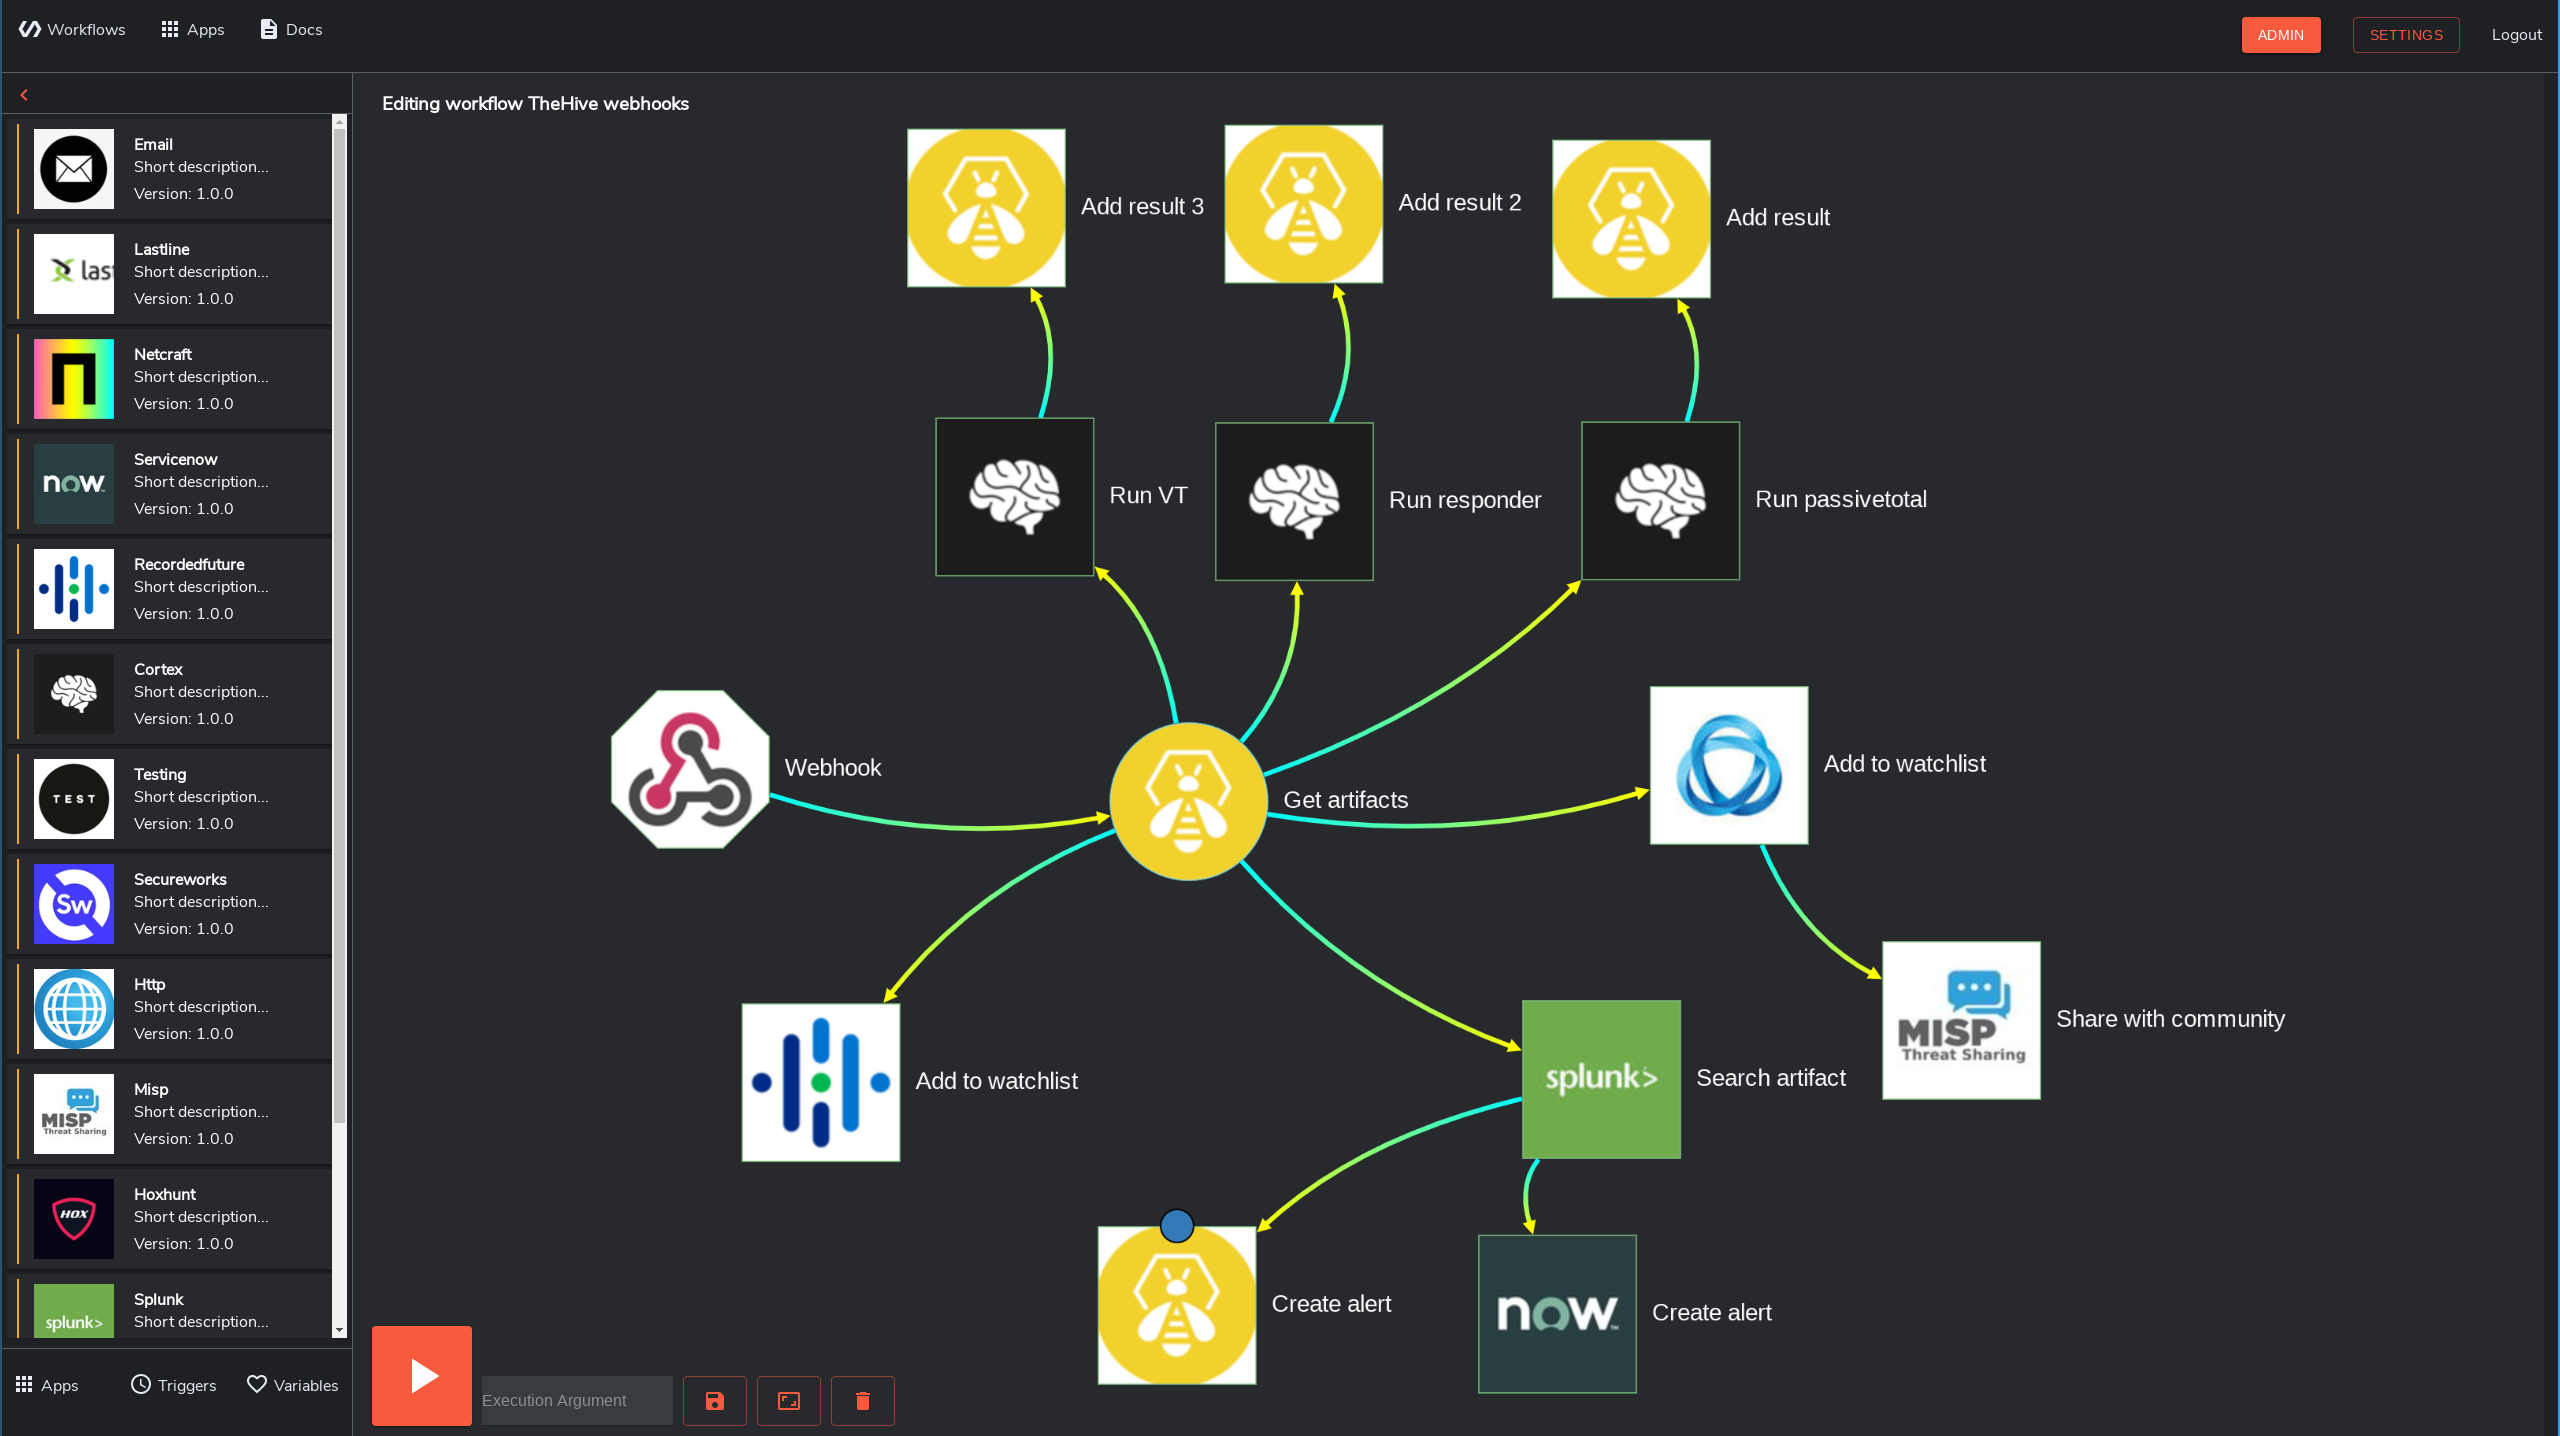
\includegraphics[width=0.9\textwidth]{images/shuffle_soar_workflow.png}
        \caption[Example of a workflow editor in Shuffle SOAR]{Example of a workflow editor in Shuffle SOAR. The visual interface allows users to design and manage automated response workflows by connecting integration actions and defining execution logic.}
    \label{fig:shuffle-soar-workflow}
\end{figure}

Palo Alto Cortex XSOAR expands this by providing conditional flows, loops, exception handling, and variable sharing, across tasks~\cite{paloalto}. Its workflow engine enables automation tasks and human-in-the-loop interactions (e.g., approval requests), providing hybrid response models.

Open source SOAR platforms, like Shuffle, are also based on workflow automation and provide a visual interface for drag-and-drop placement of integration actions, conditional paths, and data variables~\cite{techtarget}. Shuffle workflows typically reflect a preference for simplicity and ease of scripting by providing fewer limitations, safety guards, and error-handling capabilities relative to enterprise-class systems.

Overall, the workflow module turns logical response strategies into executable sequences, and establishes the structure for managing security automation as a part of the SOAR. The workflow module closes the loop from decision logic to operational execution in incident handling with regard to efficiency and auditability.

\subsection{MITRE ATT\&CK Module}

The MITRE ATT\&CK(Adversarial Tactics, Techniques, and Common Knowledge) module embeds the widely used threat modeling framework into the SOAR platform for enriched contextual awareness, incident classification, and response strategy alignment . ATT\&CK provides a canvas of an adversary's actions structured by tactics (goals) and techniques (procedures), allowing SOC teams to build the "why" and "how" behind identified threats~\cite{mitre}.

In the implemented SOAR system, the MITRE ATT\&CK module offered a visually interactive matrix interface of the ATT\&CK Enterprise Matrix. The key features of the ATT\&CK module include:

\begin{itemize}
    \item \textbf{Technique-Based Filtering:} Each cell in the matrix represents an ATT\&CK technique, which allows the user to filter and provide a list of incidents mapped to the technique with a click.
    
    \item \textbf{Heatmap Visualization:} A color heatmap will overlay the matrix to show the mapping of incidents to techniques. The heatmap will show colors from white (absence of incidents), blue (low observed frequency of incidents), and red (high observed frequency of incidents) to visually observe the most frequently observed technique in the environmental.
    
    \item \textbf{Technique-Incident Association:} When incidents are ingested, the techniques can be mapped automatically or manually to links each incident to a corresponding set of ATT\&CK entries. This classification can be utilized to help develop the investigation.
\end{itemize}

\begin{figure}[ht]
    \centering
    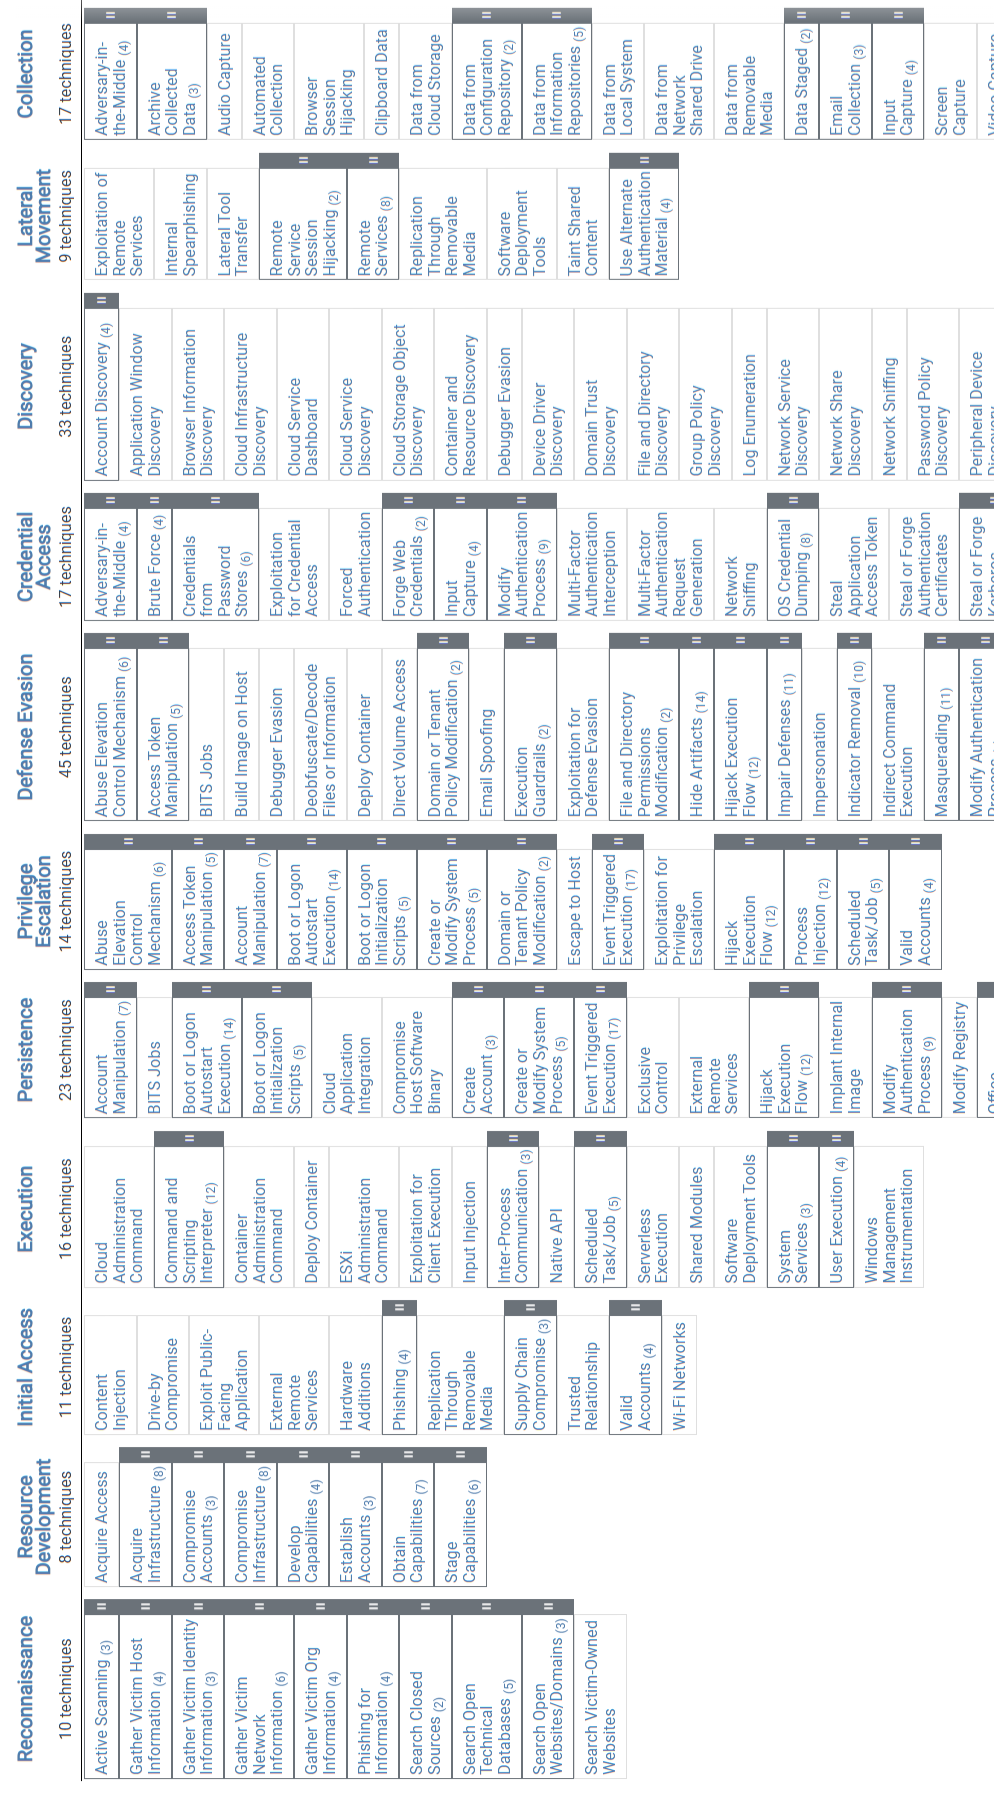
\includegraphics[width=0.9\textwidth]{images/mitre_att&ck_matrix.png}
    \caption[Interactive MITRE ATT\&CK matrix]{Interactive MITRE ATT\&CK matrix. The matrix enables analysts to visualize incident distribution across tactics and techniques, supporting rapid threat attribution and response prioritization.}
    \label{fig:mitre-attck-matrix}
\end{figure}

The integration of MITRE ATT\&CK in SOAR platforms serves multiple purposes: it enhances situational awareness, supports threat hunting, and allows for better alignment of detection and response strategies with real-world adversary tactics. Furthermore, it provides a foundation for behavioral analytics, red teaming, and compliance reporting.

Commercial SOAR tools like Palo Alto Cortex XSOAR have integration with ATT\&CK built in to the tool. Incidents can be annotated with tactics and techniques, and XSOAR has dashboard modules that allow for visualization of coverage and attack surface exposure~\cite{paloalto}. XSOAR can also leverage ATT\&CK metadata, and it supports threat intel enrichment, and filtering/reporting based on distribution of techniques. 

Splunk SOAR does not have a native ATT\&CK matrix framework, but playbooks and detections can be mapped to tactics and techniques via integration with the Splunk Security Essentials app or external visualization tools (eg, MITRE ATT\&CK Navigator)~\cite{splunk}.

Open-source platforms such as Shuffle, are not configured out-of-the-box to support an ATT\&CK framework, however, users may still tag incidents and utilize third-party tools for visualization, such as ATT\&CK Navigator, Kibana, or D3.js-based dashboards~\cite{techtarget}.

This custom SOAR platform incorporates ATT\&CK as a native component of the platform by providing a native visual matrix chart closely tied to incident metadata, and playbook execution. By embedding an ATT\&CK visualization in the SOAR platform, the analyst gains immediate insights of threat patterns, and can prioritize response actions according to frequently used techniques. This also allows for proactive defensive posture by identifying techniques that are unmonitored and under-monitored for detection and response.

Overall, the MITRE ATT\&CK matrix and reference module enhance the strategic value to the SOAR platform, enabling application of structured threat intelligence, which can better position prioritization, and increased operational alignment with adversarial behavior.